\documentclass[../../main.tex]{subfiles}

% 

\begin{document}
\chapter{Fenomenologické modely jader}

\section{Zadanie}

Jaderné síly, Deuteron, N-N potenciál, Coulombická bariéra, Mezonová teorie jaderných sil(Yukawův potenciál), Klasifikace jaderných modelů, Kapkový model jádra, Slupkový model jádra, Zobecněný model.

\section{Jaderné síly}

Modely vždy představují jakousi zjednodušenou představu zachycující vybrané vlastnosti atomového jádra. Už víme, že jádro je kvantovou soustavou nukleonů, mezi nimiž působí silná, elektromagnetická a slabá interakce. Interakce, která zajišťuje existenci jádra jako vázaného systému nukleonů, je samozřejmě interakce silná.

Nyní si shrneme základní vlastnosti projevu silné interakce v jádře, tj. JADERNÝCH SIL:
\begin{itemize}
	\item Jaderné síly jsou předně uvnitř jádra i na jeho hranicích podstatně větší než síly elektromagnetické $\rightarrow$ plyne to např. z velikosti separačních energií vnějších nukleonů ve srovnání se separačními energiemi valenčních elektronů v atomovém obalu - první z nich mají hodnotu řádově rovnou  1 až 10 $\mathrm{MeV}$, druhé jen několik $\mathrm{eV}$. Na středních vzdálenostech mají PŘITAŽLIVÝ CHARAKTER $\rightarrow$ existují vázané stavy nukleonů, pokud by jaderné síly nebyly přitažlivé, vázané stavy by existovat nemohly.
	
	\item Na malých vzdálenostech (menších než přibližně $0,6 ~\mathrm{fm}$) jsou jaderné síly ODPUDIVÉ.
	
	\item Jaderné síly jsou na rozdíl od elektromagnetických sil silami KRÁTKÉHO DOSAHU, působí výrazně do vzdálenosti $ \sim 10^{-15} ~\mathrm{m} \equiv 1 ~\mathrm{fm}$ a potom rychle klesají k nule. Fakt, že dosah jaderných sil je menší než vzdálenosti mezi atomy, lze odvodit ze skutečnosti, že na molekulární úrovni je k vysvětlení daných jevů zapotřebí pouze elektromagnetické interakce.
	
	\item U jaderných sil se projevuje NASYCENÍ. Je to jev, který je patrný z Weizs$\ddot{a}$ckerovy formule i z toho, že vazbová energie na jeden nukleon pro větší jádra prakticky nezávisí na nukleonovém čísle $A$ a má hodnotu přibližně rovnou 8 $\mathrm{MeV}$.
	
	\item U jaderných sil se setkáváme se zákonem zachování izotopického spinu a jeho projekce. Silná interakce v jádře sice závisí na velikosti izotopikého spinu, ale nezávisí na jeho projekci. To znamená, že jaderné síly jsou NÁBOJOVĚ NEZÁVISLÉ. Tvrzení lze také potvrdit existencí zrcadlových jader.
	
	Pozn.: Izospin je vnitřní stupeň volnosti se dvěma povolenými stavy $\rightarrow$ proton a neutron
	
	\item  Jaderné síly jsou ZÁVISLÉ NA SPINU. Víme totiž, že interakce mezi elektrony v atomovém obalu je na spinu závislá a oprávněně můžeme totéž očekávat u nukleonů, neboť to jsou fermiony nesoucí spin $1/2$. Tvrzení plyne také z toho, že víme o existenci vázaného stavu se spinem rovným $1$ $\rightarrow$ deuteron $~\equiv ~\uparrow\uparrow$ a přitom neexistuje vázaný stav se spinem rovným $0$ ($\uparrow\downarrow$).
	
	\item Jaderné síly jsou silami VÝMĚNNÉHO CHARAKTERU. Při interakci dochází k výměně pionů, které jsou sestaveny z mořských kvarků generovaných vakuovými excitacemi. Jako experimentální důkaz výměnnosti může posloužit symetrie diferenciálního účinného průřezu v těžišťové soustavě.
	
	\item Jaderné síly jsou obecně NECENTRÁLNÍ, jak plyne z existence elektrického kvadrupólového momentu a nesférických jader. Navíc jsou to síly tenzorového charakteru - nepůsobí mezi středy objektů, kromě vzdálenosti objektů závisejí také na úhlu mezi spiny a přímkou spojující středy objektů interakce. 
\end{itemize} 
	V kvantifikaci popisu jaderných sil nám brání skutečnost, že dosud neznáme zákon silné interakce, který by popisoval tuto interakci nějakou takovou formou, jakou je např. popsána gravitační síla. Ukazuje se totiž, že silná interakce mezi nukleony je zbytkovou silnou interakcí mezi kvarky tvořícími nukleony (je to podobný stav, s jakým se setkáváme u mezimolekulárních sil van der Waalsova typu, které jsou zbytkovými silami elektromagnetickými, udržujícími pohromadě atomy a molekuly). Tuto interakci však nemůžeme odvodit ze silné interakce  mezi kvarky, protože pro ně zákon silné interakce také neznáme.
	
	V roce 1935 navrhl Bethe, že nukleony v jádře je možné pokládat za neinteragující částice, pohybující se v potenciálové jámě, přičemž daný potenciál je vytvářen všemi ostatními nukleony. V tomto modelu bylo působení jednoho nukleonu na ostatní nukleony bráno jako působení jednoho celkového potenciálu ode všech ostatních nukleonů. Tento potenciál působí stejně na vázané i na nevázané nukleony, a tudíž je velmi jednoduché vypočítat rozptyl nukleonu na tokovém potenciálu - dostali bychom účinný průřez, jenž by byl hladkou funkcí energie příchozí částice.
	
	Avšak brzy bylo ukázáno, že účinný průřez by v tomto případě nebyl hladkou funkcí, ale měl by rezonanční strukturu. Rezonance jsou úzké, se šířkami kolem 1 $\mathrm{eV}$, a tím pádem s dobami života kolem $10^{-15} ~\mathrm{s}$, což je ale mnohem delší doba, než potřebuje částice k průchodu jádrem ( ta je $ \sim 10^{-22} ~\mathrm{s}$).
	
	Niels Bohr tedy navrhl jiný průběh reakce. Podle něj se příchozí nukleon nejdříve zachytí v jádře a vytvoří složené jádro, které žije poměrně dlouhou dobu, než se rozpadne buď elasticky zpět do původního stavu, anebo inelasticky. Příchozí částice je přitahována jádrem a interaguje silně se všemi nukleony v něm. Její energie je rozdělena mezi všechny částice, se kterými se setká, dokud není ustaven stav statistické rovnováhy. Následně se energie dále předává dalšími srážkami, dokud statistickými fluktuacemi neobdrží částice blízko povrchu jádra potřebnou energii k úniku z něj. Tento proces již trvá déle, než výše popsaný, přibližně v rozmezí $10^{-15} ~\mathrm{s}$ až $10^{-18} ~\mathrm{s}$, což odpovídá pozorovaným šířkám. 
	
	Během tohoto statistického procesu se jádro chová spíše jako kapka kapaliny (zde se totiž přeskupuje energie a probíhá vypařování z povrchu). Dynamická teorie oscilací kapky byla původně formulována Lordem Rayleighem a následně aplikována Bohrem na jaderné vibrace. Kapka je držena pohromadě povrchovým napětím, které reprezentuje vzájemné přitahování nukleonů; také může být nabitá, což vede k destabilizaci oscilací. Povrchové napětí drží kapku co nejblíže u sebe, ale Coulombická interakce se jí snaží roztrhnout $\rightarrow$ nakonec převáží Coulombická interakce a kapka se roztrhne. Tato vlastnost dělá těžká jádra nestabilní, tudíž se mohou rozpadat na dva fragmenty. Kapkový model poskytl první detailní výpočty jaderného štěpení. 
	
	Úspěch kapkového modelu zastínil dřívější Betheho model s potenciálovou jámou. Postupem času však byly objeveny jevy, které nelze vysvětlit v teorii kapkového modelu, ale které volají po modelu nezávislých částic pohybujících se v potenciálové jámě. Takový model je schopen dát magická čísla spojená se slupkovou strukturou jádra. Navíc po přidání imaginárního členu, jímž započteme tok odebraný reakcemi z elastického kanálu, se z jednočásticového modelu stane OPTICKÝ MODEL, který velmi dobře popisuje pružný rozptyl částic na jádře.    
	
\section{Coulombická bariéra}

Kromě silné interakce působí i elektrická síla. Jádro má kladný náboj a pro kladně nabitou částici vytváří tato síla COULOMBICKOU BARIÉRU $\rightarrow$ dosah elektrické síly je větší než dosah silné interakce. Příslušný potenciál má tvar
\begin{equation}
V(r) \sim Q/r.
\end{equation}

\begin{figure}[h!]
	\begin{minipage}[c]{0.5\linewidth}
		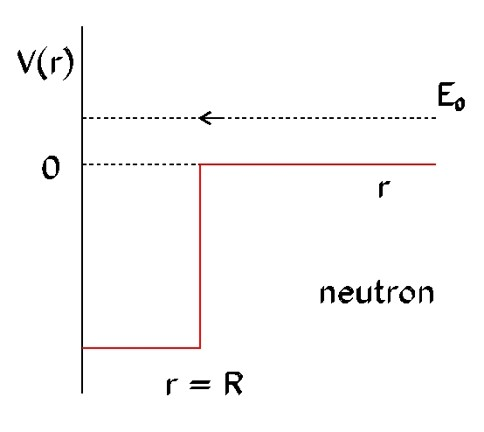
\includegraphics[width=\linewidth]{pot1.jpg}
	\end{minipage}
	\hfill
	\begin{minipage}[c]{0.5\linewidth}
		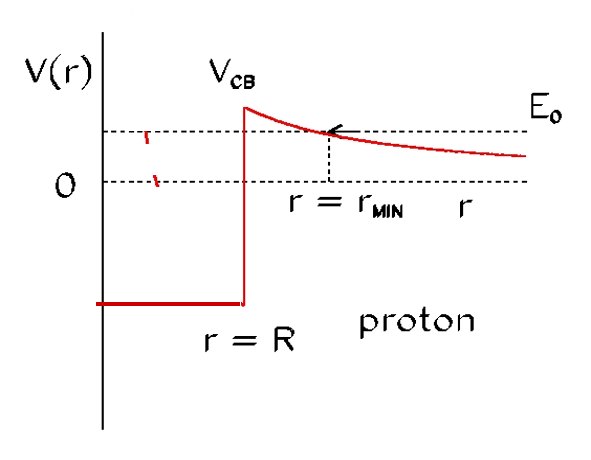
\includegraphics[width=\linewidth]{pot2.png}
	\end{minipage}
	\caption{Tvar potenciálu pro neutrony a pro protony}
\end{figure}

V případě rozptylu navíc působí ještě ODSTŘEDIVÁ BARIÉRA, která je daná momentem hybnosti nalétávající částice.

\section{Mezonová teorie jaderných sil (Yukawův potenciál)}

Výměnný charakter jaderných sil:
\begin{itemize}
	\item krátký dosah $\rightarrow$ nenulová klidová hmotnost zprostředkujících částic. Odpovídající potenciál navrhl H. Yukawa 
	\begin{equation}
	V(r) \propto \dfrac{\exp(-m c r/ \hbar)}{r},
	\end{equation}
	kde $m$ je hmotnost zprostředkující částice a $\hbar /mc$ je její Comptonova vlnová délka. Položíme Comptonovu délku rovnu dosahu $R$ jaderných sil a určíme hmotnost zprostředkující částice:
	\begin{equation}
	mc^2 = \dfrac{\hbar c}{\lambdabar} \approx  \dfrac{\hbar c}{R} = \dfrac{197 ~\mathrm{MeV.fm}}{1,7 ~\mathrm{fm}} \approx 120 ~\mathrm{MeV}. 
	\end{equation}
	
	\item Zprostředkující částice s podobnou hmotností byly nalezeny (r. 1935 Yukawa) a označeny jako MEZONY $\pi$ ($m_{\pi} = 140 ~\mathrm{MeV}$). přitažlivá a odpudivá jaderná síla je tak zprostředkována výměnou nabitých a neutrálních mezonů:
	\begin{equation}
	p+ \pi^- \rightarrow n, ~~~~ n + \pi^+ \rightarrow p, ~~~~ p + \pi^0 \rightarrow p, ~~~~ n + \pi^0 \rightarrow n 
	\end{equation}
\end{itemize}

Protony a neutrony neustále emitují a pohlcují mezony. Proč je nenacházíme s různou hmotností?

Princip neurčitosti: $\Delta E \Delta t \geq \hbar$ $\rightarrow$ nezachování energie je dovoleno, pokud trvá méně než $\hbar/\Delta E$. Maximální dosah jaderných sil je $R = 1,7 ~\mathrm{fm}$. Pak nejmenší doba přeletu nukleonu je: $ \Delta t = R/c$. Při emisi mezonu s hmotností $m_{\pi}$ se nezachovává energie: $\Delta E = m_{\pi}c^2$ . Jestliže bude doba existence nezachování energie $\Delta t$, tak pro maximální možnou energii nezachování (hmotnost mezonu) dostaneme: $m_{\pi}c^2 = \hbar c /R
$ (stejný jako výše uvedený).

Nalezeny byly i další mezony ($\eta, \rho, \phi, ...$), i dvojmezonová výměna.

\subsection{Yukawova teorie}

jaderné síly mají výměnný charakter $\rightarrow$ výměnný charakter interakce. 

\begin{center}
	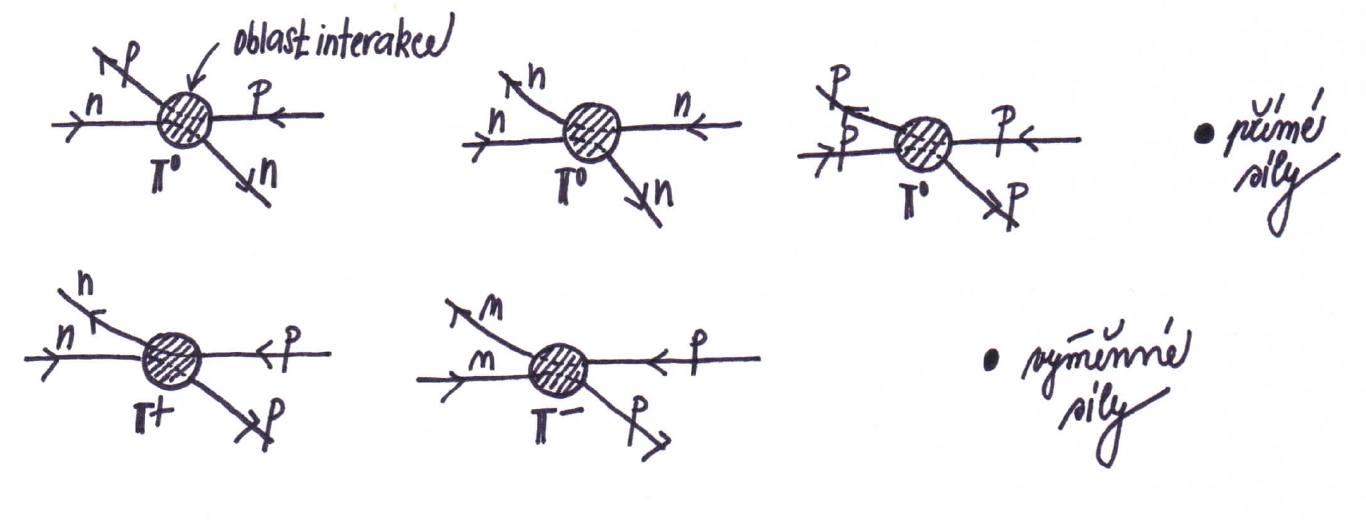
\includegraphics[width=0.9\textwidth]{vym.png}
	\captionof{figure}{Přímé síly x Výměnné síly}		
\end{center}

\begin{equation}
M_x = 0 \Rightarrow V(r) = - \dfrac{e^2}{4 \pi \epsilon_0} \dfrac{1}{r},
\end{equation}
\begin{equation}
M_x \neq 0 \Rightarrow V(r) = - \dfrac{g^2}{4 \pi } \dfrac{1}{r} \exp(-\dfrac{r}{R}); ~~~~ R = \dfrac{\hbar}{M_x c} ... \textit{dosah interakce}, g ... \textit{síla interakce}
\end{equation}
$\Rightarrow$ popisuje jaderné síly na vzdálenostech $r \geq 2 ~\mathrm{fm}$. Pro $r < 1 ~\mathrm{fm}$ nelze použít $\Rightarrow$ zanedbává vnitřní strukturu nukleonu $\Rightarrow$ QCD.

\section{N-N potenciál}

Nukleon- nukleonový potenciál:
\begin{equation}
U(r) = \dfrac{g^2}{4 \pi r} \exp (- \dfrac{mc }{\hbar} r)
\end{equation}
Z rozptylu N-N a ze stability jader $\Rightarrow$ musí existovat odpudivé jádro interakce

\begin{center}
	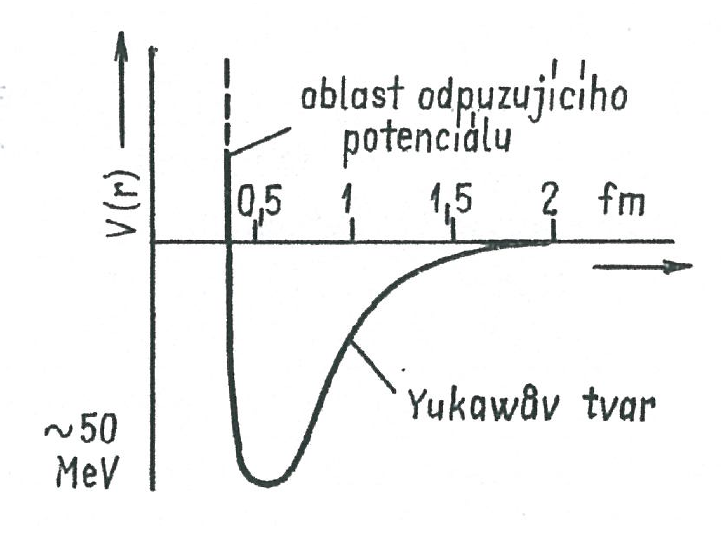
\includegraphics[width=0.5\textwidth]{poten2.png}
	\captionof{figure}{Nejjednodušší přiblížení průběhu potenciálu mezi dvěma nukleony}		
\end{center}

\begin{figure}[h!]
	\begin{minipage}[c]{0.5\linewidth}
		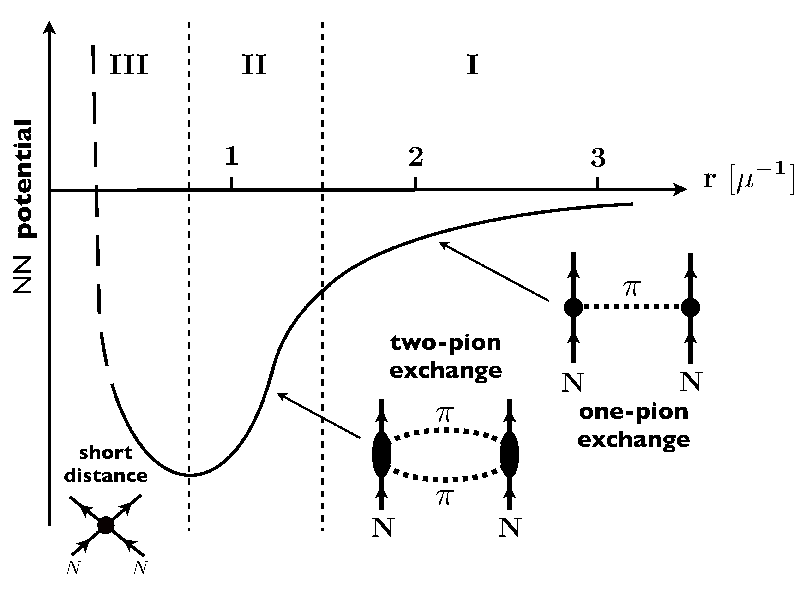
\includegraphics[width=\linewidth]{poten.png}
	\end{minipage}
	\hfill
	\begin{minipage}[c]{0.5\linewidth}
		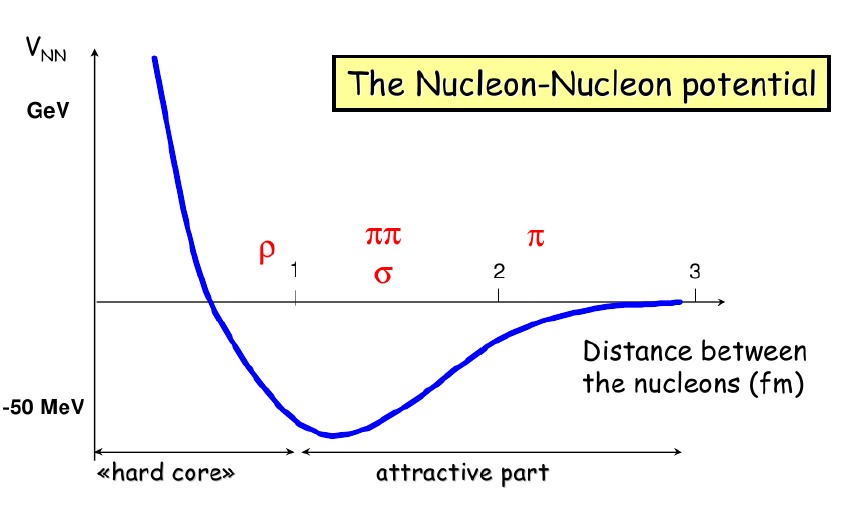
\includegraphics[width=\linewidth]{N_N.png}
	\end{minipage}
	\caption{N-N potenciál}
\end{figure}

Z požadavků základních symetrií a vlastností interakce lze sestavit\newline obecný tvar $H_{int} = (\vec{r}, \vec{p}, \vec{s}(1,2), \vec{\tau}(1,2))$.

Především:
\begin{itemize}
	\item Z analýzy deuteronu $\Rightarrow$ existuje část $H_{int}$, která nezachovává $L$ (celý $H$ ale musí zachovávat $J$ a $P$).
	
	\item silně závisí na spinu a závisí na izospinu
\end{itemize}
Možné součásti:
\begin{itemize}
	\item sféricky symetrická interakce $V(\vec{r}) = V(|r|) $ ve tvaru např. $V \sim \dfrac{1}{r^3}$ - nezachovává sice $L$, ale ani $J$ (není rotačně invariantní) $\Rightarrow$ NELZE
	
	\item tvar $V = f(r) \vec{S} \vec{r}$ - nezachovává $L$, zachovává $J$, ale nezachovává $P$ $\Rightarrow$ NELZE
\end{itemize}

Obecný tvar N-N potenciálu:
\begin{equation}
\begin{aligned}
V(r;\sigma_1, \sigma_2, \tau_1, \tau_2) & = \\ 
& = V_0(r) + V_{\sigma} (r) \vec{\sigma_1} \cdotp \vec{\sigma_2} + V_{\sigma \tau} (r) (\vec{\sigma _1} \cdotp \vec{\sigma_2}) (\vec{\tau_1} \cdotp \vec{\tau_2}) \\
& + V_{LS} (r) \vec{L} \cdotp \vec{S} + V_{LS \tau}(r) (\vec{L} \cdotp \vec{S}) (\vec{\tau_1} \cdotp \vec{\tau_2}) \\
& + V_T (r) S_{12} + V_{T \tau} (r) S_{12} (\vec{\tau_1} \cdotp \vec{\tau _2}) \\
& + V_Q(r) Q_{12} + V_{Q \tau} (r) Q_{12} (\vec{\tau_1} \cdotp \vec{\tau _2}) \\
& + V_{PP} (r) (\vec{\sigma _1} \cdotp \vec{p}) (\vec{\sigma_2 } \cdotp \vec{p} ) + V_{PP \tau} (r) (\vec{\sigma _1} \cdotp \vec{p}) (\vec{\sigma_2 } \cdotp \vec{p} )(\vec{\tau_1} \cdotp \vec{\tau_2}),
\end{aligned}
\end{equation}
kde 
\begin{equation}
Q_{12} = \dfrac{1}{2} \left[ (\vec{\sigma_1} \cdotp L) (\vec{\sigma_2} \cdotp L) + (\vec{\sigma_2} \cdotp L) (\vec{\sigma_1} \cdotp \L)\right] 
\end{equation}
\begin{equation}
S_{12} = \dfrac{3}{r^2} (\vec{\sigma_1} \cdotp \vec{r})(\vec{\sigma_2} \cdotp \vec{r}) - \vec{\sigma_1} \cdotp \vec{\sigma_2}.
\end{equation}

Deuteron $\Rightarrow$ hloubka potenciálu je $\sim 35 ~\mathrm{MeV}$.

\section{Deuteron}

Deuteron (n-p) je nejjednodušší vázaný stav nukleonů. 
\begin{itemize}
	\item vazbová energie $E_V \backsimeq 2,2 ~\mathrm{MeV}$
	\begin{itemize}
		\item reakce $p(n, \gamma)d$
		\item slabě vázaný systém
		\item žádné excitované stavy
	\end{itemize}
	\item neexistuje vázaný stav n-n, p-p
	\item spin a parita $1^+$
	\begin{itemize}
		\item možné stavy (L,S): (0,1) (2,1)
	\end{itemize}
	\item 	izospin $T_z = 0$
	\begin{itemize}
		\item žádné vázané stavy n-n, p-p (stavy s $T_z = 0, T_z = 1$) $\Rightarrow$ $T=0 $ pro deuteron - závislost N-N potenciálu na izospinu
	\end{itemize}	
\end{itemize}
Chceme fenomenologicky najít tvar potenciálu $V_{NN} (\vec{x_i}, \vec{p_i}, \vec{L}, \vec{S_i}, T_i, ...)$ který bude splňovat tyto požadavky

\subsection{Vazebná energie}

Nejjednodušší aproximace - sférická jáma, která musí pojmout jen jeden vázaný stav $\Rightarrow$ známe šířku $\sim 2 ~\mathrm{fm} $ $\Rightarrow$ $V_0 \sim 35 ~\mathrm{MeV}$.

\subsection{Spin a parita deuteronu}

\begin{center}
	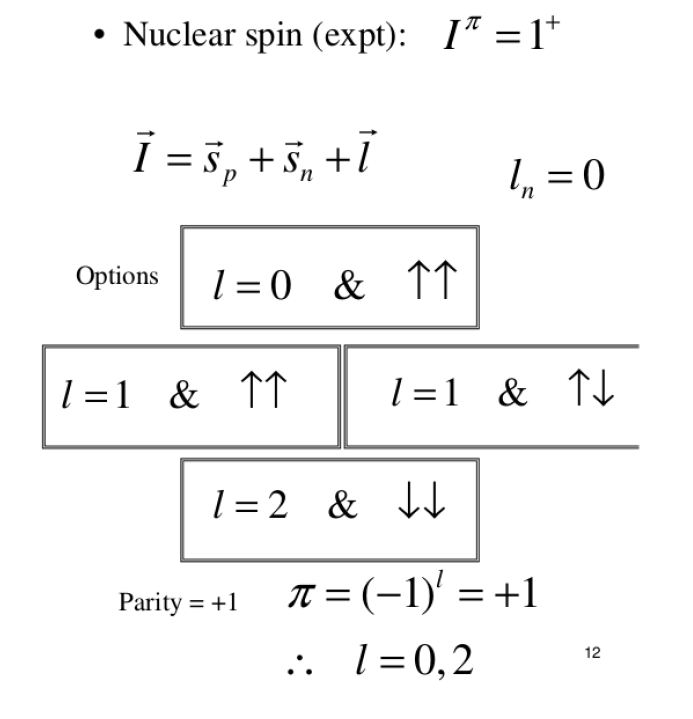
\includegraphics[width=0.5\textwidth]{spin.png}
	\captionof{figure}{Spin a parita deuteronu}		
\end{center}

\subsection{Spinová závislost silné interakce}

Neexistuje žádný  vázaný stav $I=0$, nebo $1^{-}$ - tj. antiparalelní spiny
\begin{itemize}
	\item d = p + n
	\begin{equation}
	S_p = \dfrac{1}{2} ~~~~~~~~~~~ S_n = \dfrac{1}{2}  ~~~ \Rightarrow \vec{S_d} = \vec{S_p} + \vec{S_n}
	\end{equation}
	
	\item možnosti jsou: $S_d  = 0 ~~ (\uparrow \downarrow)	 ~~~~~~~~ S_d = 1 ~~ (\uparrow \uparrow)$
	
	\item experimentálně, deuteron má pouze jeden vázaný stav s $S_d = 1$
	
	\item takže, silná interakce je spinově závislá
\end{itemize}

\subsection{Magnetický dipólový moment deuteronu}

Je to příspěvek dipólových momentů nukleonů a příspěvek orbitálního pohybu $\Rightarrow$
\begin{equation}
\mu ^{\vec{spin}} = g_S \mu _N \vec{s}
\end{equation}
\begin{equation}
\mu ^{\vec{orbit}} = g_L \mu _N \vec{l}.
\end{equation}
\begin{itemize}
	\item orbitální g-faktory: $g_L = 0 ... neutron$, ~~ $g_L = 1 ... proton$
	\item spinové g-faktory: $g_S = - 3,826085 ... neutron$, ~~ $g_S = 5,585695 ... proton$
	\item Jak to poskládat do celkového izospinu deuteronu?
	
	$\Rightarrow$ $g_{deut} = 0,857438230$ 
	\begin{equation}
	\vec{\mu} _{deut} = g_n \mu _N \vec{s}_n + g_p \mu _N \vec{s}_p + \dfrac{1}{2} \vec{L}.
	\end{equation}
	\end{itemize}

$^{3}S_1 $ stav (tj. l=0, s=1): 
\begin{equation}
\mu _{deut} = \mu_p + \mu _n = 0,8798 \mu _N,
\end{equation}
\begin{equation}
\mu _{deut} - \mu _{deut} (^{3} S_1) = - 0,022367 \mu _N.
\end{equation}
	
Nestačí vysvětlit celkový dipólový moment
\begin{itemize}
   \item musí existovat příspěvek od stavů s $l\neq 0$
   \item musí existovat necentrální komponenta interakce, která nezachovává orbitální moment hybnosti
   \item deuteron je superpozice stavů s různým $l$
 \end{itemize}  	
 
 Z předchozí analýzy spinu a parity $\Rightarrow$ lze mixovat jen s $^{3}D_1$ stavem (L=2, S=1):
 \begin{equation}
 \psi _{deut} = a \psi (^{3}S_1) + b \psi (^{3}D_1),
 \end{equation}	
 kde 
 \begin{equation}
 a^2 \simeq 0,96 ~~~~~ b^2 \simeq 0,04.
\end{equation}

\subsection{Kvadrupólový moment deuteronu}

Deuteron má nenulový kvadrupólový moment $Q \neq 0$ $\rightarrow$ nemůže být v čistém $l=0$ stavu
\begin{equation}
\psi _d = a \psi (^{3}S_1) + b \psi (^{3}D_1),
\end{equation}
kde z hodnot  mag. dip. momentu a kvadrup. momentu dostaneme $b^2 = 0,5 - 0,7$, což souhlasí s hodnotou získanou z analýzy mag. dip. momentu. Musí existovat tenzorová složka potenciálu
\begin{equation}
S_{12} = \dfrac{3}{r^2} (\vec{\sigma_1} \cdotp \vec{r})(\vec{\sigma_2} \cdotp \vec{r}) - \vec{\sigma_1} \cdotp \vec{\sigma_2},
\end{equation}
$\Rightarrow$ vl. stavy nezachovávají ostrou hodnotu $L$.

\section{Klasifikace jaderných modelů}

\subsection{Proč používáme modely atomových jader?}

V současné době neexistuje jednotná teorie jaderných sil. To má za následek, že neumíme uspokojivě vysvětlit všechny mnohotvárnosti jevů a vlastnosti atomových jader. Nedovedeme např. odpovědět na tyto otázky:
\begin{itemize}
	\item 1. Jaká jádra jsou stabilní? Jaká jsou radioaktivní? Jaké jsou druhy radioaktivity? Jaký je u radioaktivních jader poločas rozpadu, tvar spektra, úhlové rozdělení emitovaných částic?
	
	\item 2. Čemu je pro libovolné jádro roven poloměr, hmotnost, vazbová energie, spin, magnetický dipólový moment, parita, elektrický kvadrupólový moment a další charakteristiky?
	
	\item 3. V jakých energetických se může nacházet dané atomové jádro? Jaké hodnoty energie, spinu, magnetického dipólového momentu, parity atd. přísluší těmto energetickým stavům?
	
	\item 4. Čemu jsou rovny pravděpodobnosti přechodů z vyšších energetických stavů do nižších?
	
	\item 5. Jak se mění účinné průřezy různých částic s různými jádry v závislosti na energii?
\end{itemize}

Neznalost teorie jaderných sil nutí fyziky k zavádění různých modelů. Modelem rozumíme jednoduchou představu zachycující některé vybrané vlastnosti atomového jádra, které jsou hlavní pro vytvoření daného modelu. Jiné vlastnosti jádra se v tomto modelu zanedbávají. 

Je přirozené, že model jádra vytvořený na tomto principu má omezenou oblast použití. Avšak v mezích této oblasti dovoluje každý model získat řadu zajímavých výsledků. Neexistuje tak zatím univerzální model, jenž by správně popisoval všechna experimentální data. 

Modely atomových jader jsou fenomenologické teorie, jež berou existenci jaderných sil a jejich vlastností (alespoň nejdůležitější) jako daný fakt a nesnaží se studovat jejich podstatu.

Modely dělíme do dvou skupin:
\begin{itemize}
	\item KOLEKTIVNÍ MODELY - modely respektující silnou interakci mezi nukleony a pokládající jádro v podstatě za jeden celek $\rightarrow$ kapkový model
	
	\item JEDNOČÁSTICOVÉ MODELY - modely nezávislých částic považující nukleony za navzájem nezávislé částice pohybující se v jistém středním potenciálovém poli, které samy vytvořily $\rightarrow$ slupkový model, model Fermi-Diracova plynu, optický model
\end{itemize}

Přechod mezi oběma skupinami tvoří tzv. ZOBECNĚNÝ MODEL ATOMOVÉHO JÁDRA. Tento model přihlíží jak k pohybu individuálních částic v jistém středním potenciálovém poli, tak i ke kolektivnímu pohybu velké skupiny nukleonů (rotaci a deformaci jádra beze změny objemu).

\section{Kapkový model jádra}

Jaderná hmota má dvě vlastnosti, které jsou velmi shodné s kapkou kapaliny. Těmito vlastnostmi jsou konstantní vazebná energie na jeden nukleon a konstantní hustota jaderné hmoty. Tato analogie vedla k vytvoření kapkového modelu atomového jádra a formulaci semi-empirické Bethe-Weizs$\ddot{a}$ckerovy formule.

KAPKOVÝ MODEL je jedním z elementárních modelů atomových jader, v němž se jádro považuje za kapku těžko stlačitelné kapaliny držené pohromadě nasycenými silami krátkého dosahu. Tato představa vede bezprostředně k úměrnosti mezi objemem jádra a počtem nukleonů, které se v něm nacházejí. Poloměr jádra by měl proto být dán vztahem
\begin{equation}
R = r_0 A ^{1/3},
\end{equation}
v němž konstantu $r_0$ určíme na základě srovnání vypočtených výsledků s experimentálními daty. Optimální hodnota $r_0$ se pohybuje kolem $1,3 ~\mathrm{fm}$. Dále uvedeme Bethe-Weizs$\ddot{a}$ckerovu formuli, která udává závislost vazbové energie jader na číslech $A$ a $Z$
\begin{equation}\label{sf7:eq:7.1}
B(A,Z) = a_v A - a_s A^{2/3} - a_c \dfrac{Z^2}{A^{1/3}} - a_a \dfrac{(A - 2Z)^2}{A} \pm \delta,
\end{equation}
kde 
\begin{equation}
\delta = \dfrac{a_p}{A^{1/2}}
\end{equation}
a nabývá hodnot $+ \delta$ pro sudo-sudá jádra, $- \delta$ pro licho-lichá jádra a 0 pro sudo-lichá nebo licho-sudá jádra. 

Konstanty nabývají hodnot
\begin{equation}
a_v = 15,85 ~\mathrm{MeV}, ~~~ a_s = 18,34 ~\mathrm{MeV}, ~~~ a_c = 0,71 ~\mathrm{MeV}, ~~~ a_a =23,7 ~\mathrm{MeV}, ~~~ a_p = 11,5 ~\mathrm{MeV}. 
\end{equation}

Vezmeme-li v úvahu vztah $R = r_0 A^{1/3}$ mezi poloměrem jádra a hmotnostním číslem, pak vidíme, že první člen ve vztahu (\ref{sf7:eq:7.1}) je OBJEMOVÁ ENERGIE jádra, která je podstatná pro vytvoření kapky (tento první člen také můžeme nazvat "vazbovou energií", kterou následujícími členy budeme korigovat). Druhý člen je úměrný POVRCHU JÁDRA a vystihuje skutečnost, že nukleony na povrchu jsou méně vázané, neboť interagují s menším počtem nukleonů než nukleony uvnitř kapky (stejně jako u kapky kapaliny je u jádra povrchové napětí projevem slabší vazby u povrchu). Třetí člen reprezentuje COULOMBICKÉ ELEKTROSTATICKÉ ODPUZOVÁNÍ PROTONŮ, odpudivá síla mezi protony snižuje vazbovou energii; Pro rovnoměrně nabitou kouli je Coulombovská energie $E \propto Q^2 /R$, pro jádro $Q^2 = Z^2 e^2 $. Čtvrtý člen je nazývaný ASYMETRICKÝM ČLENEM, je to fenomenologický člen a vystihuje skutečnost, že stabilní nuklidy leží na linii stability, tj. že přibližně platí $N = Z$. Poslední příspěvek se rovněž nedá dobře objasnit v rámci kapkového modelu, neboť souvisí zejména se spinovými , ale také s izospinovými stavy systému nukleonů; nazývá se PÁROVÝ ČLEN a odráží skutečnost, že dva protony nebo dva neutrony jsou vždy silněji vázány než jeden proton nebo jeden neutron. Efekty jednotlivých členů na celkovou vazebnou energii jednoho nukleonu v jádře jsou na následujícím obrázku.


\begin{center}
	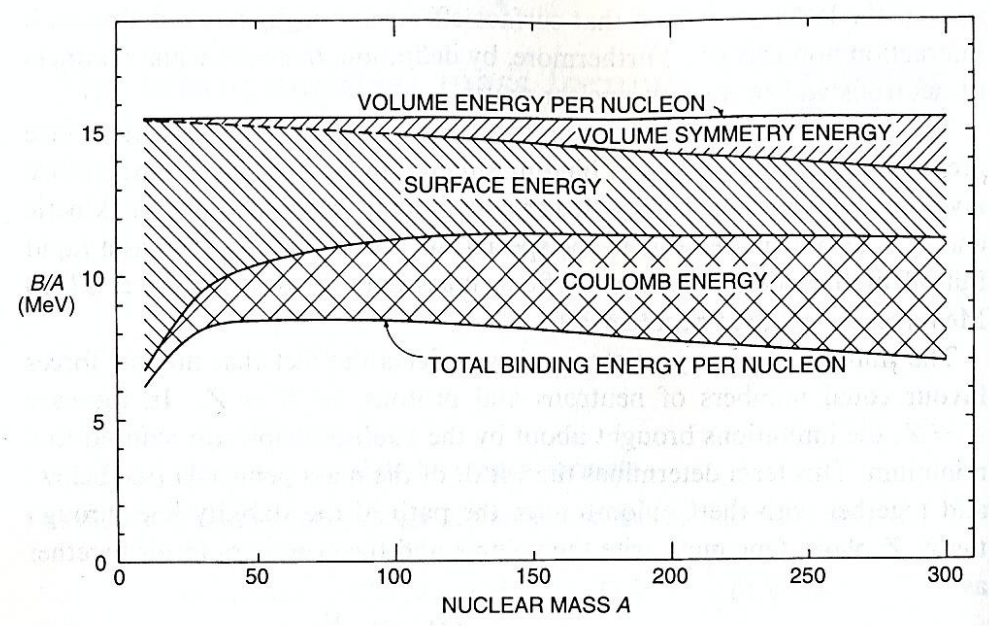
\includegraphics[width=0.8\textwidth]{Bethe.png}
	\captionof{figure}{Efekt jednotlivých členů v Bethe-Weizs$\ddot{a}$ckerovy formuli na vazebnou energii na jeden nukleon}		
\end{center}

Ještě pár poznámek ke čtvrtému členu v BW formuli, který zahrnuje asymetrii mezi počtem protonů a neutronů v atomovém jádře. V tichosti jsme předpokládali, že jakmile jsou efekty Coulombického odpuzování mezi protony zahrnuty do jiného členu v BW formuli, vazba protonů je stejná jako vazba neutronů. Představme si tedy dvě identické potenciálové jámy zvlášť pro protony a neutrony. Energetické úrovně v těchto jámách se zaplňují v souladu s Pauliho vylučovacím principem, jelikož protony i neutrony jsou fermiony. Pokud platí $Z=N$, jsou obě jámy zaplněny do stejné úrovně (Fermiho hladina). Jakmile se ale z této situace přesuneme do stavu, kdy $N>Z$, musí být jeden proton zaměněn za neutron, tj. přejít na volnou neutronovou slupku. Tento stav tak má energii o $\Delta E$ vyšší než původní stav ($\Delta E$ je rozdíl mezi energiemi dvou sousedících hladin). Druhý podobný krok se záměnou protonu a neutronu zvýší energii tohoto stavu opět o $\Delta E$, takže vzhledem k původnímu stavu je energetický rozdíl už 2 $\Delta E$. Záměna dalšího protonu v neutron zvýší energii již o $3 \Delta E$, celková změna je tak $5 \Delta E$ atd.

Tudíž změna z $Z=N$ na $N>Z$ při $A = N+Z$ konstantním vyžaduje energii $\sim (N-Z)^2 \Delta E/8$. tato změna je samozřejmě nezávislá na tom, jestli zaměníme protony v neutrony nebo naopak. Vidíme tedy, že jádra, pro něž platí $Z=N$, mají méně energie a jsou tedy silněji vázány než jádra s $Z \neq N$. Abychom tento fakt zahrnuli do BW formule, přidáváme asymetrický člen, který redukuje vazebnou energii pro jádra s $Z \neq N$. 

\begin{center}
	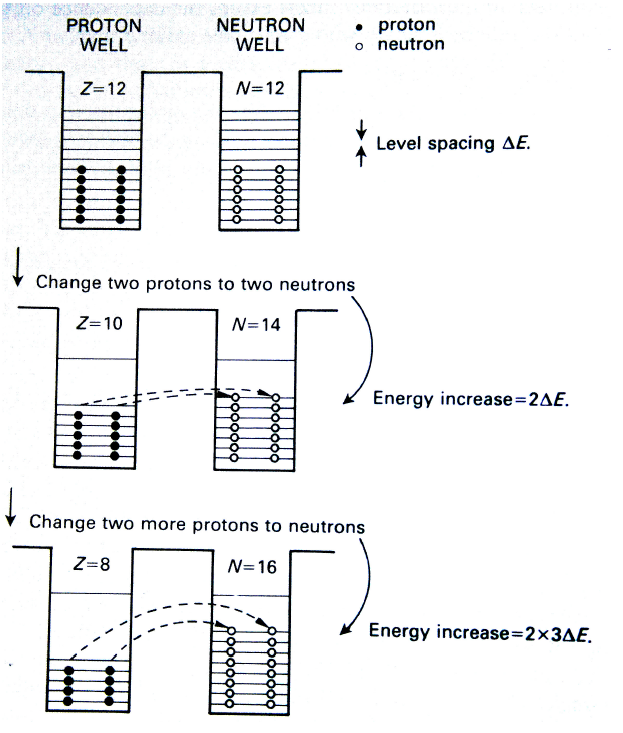
\includegraphics[width=0.6\textwidth]{kapk.png}
	\captionof{figure}{Ilustrace k zavedení asymetrického členu v Bethe-Weizs$\ddot{a}$ckerově formuli}		
\end{center}

Kapkový model lze dobře použít pro orientační výpočet hmotnosti atomového jádra $m(A,Z)$, tj.
\begin{equation}
m(A,Z) = Z m_p + (A -Z)m_n - \dfrac{B(A,Z)}{c^2},
\end{equation}
či vazebné energie $B(A,Z)$, přičemž odchylka hodnoty vazebné energie vypočtená BW formulí od experimentální hodnoty nepřesahuje 20 $\mathrm{MeV}$.

Dále tento model také dovoluje výpočet energie rozpadu $\alpha$ (je to také záporná hodnota separační energie)
\begin{equation}
Q_{\alpha} = \left[ m(A,Z) - m(A-4,Z-2) - m(^{4}_{2}He)\right] c^2 = E(A-4, Z-2) - B(A,Z).
\end{equation}
Také pomocí něj můžeme formulovat kvalitativní teorii štěpení, kde energie štěpení je dána vtahem
\begin{equation}
E_t = \left[ m(A,Z) - 2m (\dfrac{A}{2}, \dfrac{Z}{2})\right] c^2 = a_s A^{2/3} (1 - 2^{1/3}) + a_c \dfrac{Z^2}{A^{1/3}} (1 - 2^{1/3}) = - 5,12 A^{2/3} + 0,284 \dfrac{Z^2}{A^{1/3}},
\end{equation}
přičemž pro stabilní jádra až do $A\approx90$ je tato veličina záporná. Pro $Z^2/A \geq 17$ je energeticky možné štěpení, pro $Z^2 /A \geq 45$ je možné samovolné štěpení.

Předností kapkového modelu je jeho jednoduchost, názornost a snadné matematické zpracování. Z kapkového modelu vychází Bethe-Weizs$\ddot{a}$ckerova formule, která dává dostatečně přesné hodnoty vazbové energie (nebo hmotnosti) velkého počtu atomových jader i přesto, že v ní vystupuje pouze několik empiricky určených konstant. Tato okolnost činí formuli velmi užitečnou pro analýzu různých vlastností jader.

Jádro jako kapka však představuje pouze hrubý obraz skutečných poměrů v jádře. Nepřihlíží se ke kvantovým vlastnostem nukleonů, a proto kapkový model nevysvětluje takové důležité vlastnosti atomových jader jako je spin a parita (zákl. stavu stejně jako excit. stavů), mag. dipólový moment, hustotu jádra. Nevysvětluje ani existenci magických čísel. K vysvětlení budou potřeba jiné modely. 

Předpoklad sférických atomových jader (analogie se sférickou kapkou) znamená nulový el. kvadrupólový moment. U spousty atomových jader je ale tento moment nenulový $\rightarrow$ sféričnost jádra.

Z BW formule můžeme odvodit průběh linie stability. Při rozpadu $\beta$ se nemění $A$. Pro jádra s lichým $A$ leží hmotnosti na parabole a existuje jen jeden stabilní izotop. Pro jádra se sudým $A$ jsou díky párovému členu $\pm \delta$ tyto paraboly dvě $\rightarrow$ může existovat více stabilních izotopů. Nejstabilnější jádro v řadě izobarů:
\begin{equation}
\left( \dfrac{\partial M(A,Z)}{\partial Z}\right)_{A = konst} = 0. 
\end{equation}
Po provedení derivace
\begin{equation}
m_p - m_n + 2Z_0 a_c A^{-1/3} + 2 a_a (Z_0 - A/2)A^{-1} = 0.
\end{equation}
A odtud
\begin{equation}
Z_0 = \dfrac{A}{2} \left( \dfrac{m_n - m_p + a_a}{a_c A^{2/3} + a_a}\right) = \dfrac{A}{1,98 + 0,0155 A^{2/3}}.
\end{equation}
Z kapkového modelu lze získat i popis vibrací a rotací jádra:

Jaderná hmota je prakticky nestlačitelná, ovšem lehce lze dosáhnout povrchových vibrací, kvadrupólových - jádro se mění ze stlačeného na protažený elipsoid, oktupólových - deformace má hruškovitý tvar.

Energie vibračního stavu závisí na frekvenci:
\begin{equation}
E_{kvadr} = n_{kvadr} \hbar \omega ~~~~~~~~~~~~~~~~~~~~~~~~~~ E_{oktup} = n_{oktup} \hbar \omega,
\end{equation}
kde $n_{kvadr}, n_{oktup}$ je počet příslušných kvant. Kvadrupólové kvantum má spin $J = 2$ a oktupólové $J =3$. Speciálními vibracemi jsou nezávislé kmity protonové a neutronové kapky - gigantické dipólové rezonance. 

Pro deformovanou kapku je tu možná i rotace. Popis rotačních stavů je dán vztahem:
\begin{equation}
E_{rot} = \dfrac{\hbar ^2}{2 J} I(I+1),
\end{equation}
kde $J$ je moment setrvačnosti  a spin $I = 0,1,2,...$.

\section{Jednočásticové modely atomových jader}

Pokud budeme chtít popisovat jádro obsahující více než dva nukleony, uvědomíme si podstatný rozdíl mezi strukturou atomu a strukturou jádra. Zatímco atom má těžké centrální jádro, v jehož poli se pohybují elektrony, jádro takové centrum nemá. U atomů se při vyšetřování energetických stavů jejich obalu a jejich spekter celkem dobře osvědčila jednoelektronová aproximace, která dokonce mohla sloužit jako východisko pro přesný výpočet těchto stavů i spekter. 

Vzhledem k tomu, že důležitou úlohu v jednoelektronové aproximaci mělo právě význačné postavení jádra, může se zdát použití této myšlenky na jádro, tj. konstrukce jednočásticového modelu jádra za nedostatečně podloženou ideu. Avšak při vyšetřování jiných soustav bez rozhodujícího centra (zejména krystalů) se jednočásticové přiblížení osvědčilo.

Při popisu atomového jádra jednočásticovým modelem se nebudeme na jádro dívat jako na systém částic, které spole navzájem interagují, nýbrž jako na objekty, které vytvářejí jisté středované potenciální pole, ve kterém se všechny pohybují nezávisle na sobě. Toto pole jim nedovolí, pokud bude jádro stabilní, aby ho opustily. Pole bude tedy tvořit poteciálovou jámu, jejíž rozměry, hloubku a tvar je nutné zvolit tak, aby model byl schopen realisticky popisovat a případně i vykládat ty vlastnosti jader, o něž se zajímáme.

\subsection{Model Fermi-Diracova plynu}

K nejjednodušším a také nejstarším modelům patřícím do skupiny jednočásticových modelů atomového jádra patří FERMI-DIRACŮV MODEL. Ten se dívá na jádro jako na nukleonový plyn uzavřený v nekonečně hluboké potenciálové jámě, přičemž jednotlivé nukleony spolu vůbec neinteragují. Nekonečná hloubka jámy je pochopitelně aproximací, avšak osvědčila se. Dno jámy v tomto ohledu považujeme za hladké a od něj odečítáme energii jádra.

Ve statistickém modelu budeme mít především na mysli jádra, která budou velká. Tento model nám usnadní vytvořit si představu o vztahu mezi skutečnou hloubkou jámy a jejími rozměry. Co se týče energetických hladin, ve statistickém modelu jsou tyto hladiny relativně blízko u sebe a při velkém počtu nukleonů lze považovat energetické spektrum prakticky za spojité.

Nukleony jsou fermiony (mají spin $1/2$). Podle Pauliho vylučovacího principu může být v jednom stavu jenom jeden fermion. V potenciálu jádra existují stavy charakterizované pevně danými diskrétními hodnotami energie a momentu hybnosti. V základním stavu jsou nukleony obsazeny všechny nejnižší stavy Pauliho principem. Takový systém fermionů nazýváme DEGENEROVANÝM FERMIONOVÝM PLYNEM $\rightarrow$ nukleony nemohou změnit svůj stav (všechny jsou obsazeny) $\rightarrow$ nemohou se srážet a chovají se jako neinteragující částice.

Systém $N$ fermionů v objemu $V$ a při teplotě $T$:

Pravděpodobnost výskytu fermionu ve stavu s energií $E$:
\begin{equation}
F(E) = \dfrac{1}{1 + \exp ^ (\dfrac{E - E_F}{kT}) },
\end{equation}
kde $k$ je Boltzmanova konstanta a $E_F$ je Fermiho energie.

Určíme Fermiho hybnost $p_F$ (nerelativistické přiblížení $E_F = p_{F}^2 /2m$):\par
Zavedeme fázový prostor: rozšíření souřadnicového prostoru o prostor hybností (6 - rozměrný prostor). Element prostoru je:
\begin{equation}
dV = dx.dy.dz \rightarrow dV = d^3 r = r^2 \sin \vartheta dr d \vartheta d \varphi.
\end{equation}

Pokud není úhlová orientace důležitá, integrujeme přes úhly: 
\begin{equation}
dV = 4 \pi r^2 dr.
\end{equation}

Analogicky pro element prostoru hybností:
\begin{equation}
dV_p = d^3 p =dp_x dp_y dp_z = 4 \pi p^2 dp.
\end{equation}
Fázový prostor: $dV_{TOT} = dV . dV_p$

Z Heisenbergova principu neurčitosti: 
\begin{equation}
\Delta p_x \Delta x \geq \hbar ~~~~~ \Delta p_y \Delta y \geq \hbar ~~~~~ \Delta p_z \Delta z \geq \hbar 
\end{equation}

Objem $dV_{TOT}$ elementární buňky ve fázovém prostoru je $h^3$. V objemu $V$ je počet $d \nu$ elementárních buněk s jednou částicí s hybností $(p, p+\Delta p)$: 
\begin{equation}
d \nu = \dfrac{V 4 \pi p^2 dp}{h^3}.
\end{equation}

Nukleony mají $s=1/2$ $\rightarrow$ v každé buňce $g_s = (2s + 1) = 2$. Při $T=0$:
\begin{equation}
N = \int_{0}^{p_F} g_s d \nu  = \int_{0}^{p_F} 2 \dfrac{V 4 \pi p^2}{h^3} dp = \dfrac{8 \pi V p_{F}^3}{3 h^3},
\end{equation}
při $p < p_F$ $\rightarrow$ v buňce 2 částice, pro $p>p_F$ $\rightarrow$ v buňce 0 částic a tedy:
\begin{equation}
p_F = h \left( \dfrac{3N}{8 \pi V}\right)^{1/3} = \hbar  \left( \dfrac{3 \pi^2 N}{V}\right) ^{1/3}.  
\end{equation}
Fermiho plyn je degenerovaný pro $E_F >> kT$. Pro $E_F << kT$ $\rightarrow$ klasický plyn a Maxwellovo rozdělení.

Jádro je směs dvou degenerovaných fermionových plynů:

$Z$ protonů a $N$ neutronů uzavřených v objemu $V = (4/3) \pi R^3 = (4/3) \pi r_0 ^3 A$. Fermiho energie pro neutrony a protony v jádře:
\begin{equation}
E_F (n) = \dfrac{\hbar ^2}{2 m_n} \left( \dfrac{3 \pi^2 N}{V}\right)^{2/3} ~~~~~~~~ E_F(p) = \dfrac{\hbar ^2}{2 m_p} \left( \dfrac{3 \pi^2 Z}{V}\right)^{2/3} 
\end{equation}  
v prvním přiblížení: $m_n \approx m_p = m, Z \approx N \approx A/2$:
\begin{equation}
E_F(n) \approx E_F (p) = E_F \approx \dfrac{\hbar ^2 }{2 m r_{0} ^2} \left( \dfrac{9 \pi}{8}\right) ^{2/3} \approx 37 ~\mathrm{MeV} .
\end{equation}

Hloubka potenciálové jámy (vazba posledního nukleonu je $B/A$):
\begin{equation}
V_0 \approx E_F + B/A \approx 37 ~\mathrm{MeV} + 8 ~\mathrm{MeV} \approx 45 ~\mathrm{MeV}.
\end{equation}

Dále lze spočítat celkovou kinetickou energii:
\begin{equation}
E_{KIN} (N) = \sum_{\alpha = 1}^{N} E_{KIN, \alpha} = \int_{0}^{p_F (N)} \dfrac{p^2}{2 m} \left( 2 \dfrac{V 4 \pi p^2}{h^3} \right) dp = \dfrac{3}{5} N E_F (n) .
\end{equation}

Odtud pro $A = Z + N$ nukleonu: 
\begin{equation}
E_{KIN} (A) = \sum_{\alpha = 1}^{A} E_{KIN, \alpha} = \dfrac{3}{5} \left[ N E_F (n) + Z E_F (p) \right] .
\end{equation}

Střední kinetická energie na $A$ (pro $Z \approx A$): 
\begin{equation}
E_{KIN} (A)/A \approx \dfrac{3}{5} A E_F /A  \approx \dfrac{3}{5} E_F \approx 22 ~\mathrm{MeV}.
\end{equation}

Poznamenejme, že jádro popsané statistickým modelem bude existovat v základním stavu, pokud bude jeho teplota $T=0 ~\mathrm{K}$. Při excitaci se jeden nebo více nukleonů dostanou nad Fermiho hladinu, teplota jádra $T$ bude v takovém případě větší než nula. 

Pro kvantově-mechanický výpočet předpokládejme, že jádro je krychle o hraně $a$, a tudíž zaujímá objem $\Omega = a^3$. Tím pádem hledáme řešení Schr$\ddot{o}$dingerovy rovnice
\begin{equation}
\Delta \psi = + \dfrac{2m E}{\hbar ^2} \psi = 0,
\end{equation} 
kde $E$ je energie částice v krychli. Navíc jsou dány okrajové podmínky $\psi = 0$ na hranách této krychle. 

Požadované řešení rovnice
\begin{equation}
\psi (x,y,z) \propto \sin(k_x s) \sin (k_y y) \sin(k_z z)
\end{equation}
pro $k_x a = n_x \pi, k_y a = n_y \pi, k_z a = n_z \pi$, kde $n_x, n_y, n_z \in N^+$, splňuje okrajové podmínky. Každá uspořádaná trojice kladných přirozených čísel odpovídá právě jednomu řešení s energií $E$ a hybností $p = \hbar k$
\begin{equation}
E(n_x,n_y,n_z) = \dfrac{\hbar ^2}{2m} (k_{x}^2 + k_{y}^2 + k_{z}^2) = \dfrac{\hbar ^2 k^2}{2m}.
\end{equation}

Pokud budeme reprezentovat tato řešení 3-dimenzionálním polem bodů se souřadnicemi $(n_x, n_y, n_z)$, uvidíme, že tyto body leží na povrchu oktantu koule. Počet stavů s hybností mezi $\hbar (k; k + dk)$ je tedy 
\begin{equation}
dn = 4 \dfrac{1}{8} 4 \pi k^2 dk \left( \dfrac{a}{\pi}\right) ^3, 
\end{equation}
kde faktor 4 je kvůli spinové degeneraci a dvěma druhům nukleonů a poslední člen pochází z požadavku, aby zde bylo pouze jedno přípustné řešení pro každou krychli o hraně $\pi/a$, což pochází z $k_x a = n_x \pi$ atd. Použitím $a^3 = \Omega $ dostaneme stejný výsledek jako při klasickém  postupu. 


\begin{center}
	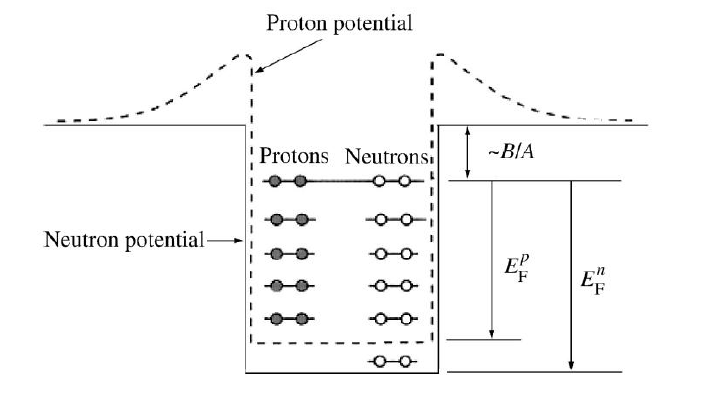
\includegraphics[width=0.8\textwidth]{fermi.png}
	\captionof{figure}{Protonové a neutronové potenciály a stavy ve Fermiho plynovém modelu}		
\end{center}

Pozn.: Fermiho kinetická energie pro protony: $T_{p,F} \dot{=} 30 ~\mathrm{MeV}$.

\section{Slupkový model jádra}

Statistický model nerespektuje dostatečně kvantový charakter systému nukleonů, nelze z něj získat např. představu o magických číslech. Touto otázkou a  s ní spojenými problémy se zabývá slupkový model atomového jádra, který ukazuje, že v systému nukleonů se setkáváme s jevem velmi blízkým uspořádání elektronů do slupek v obalu atomů, což je ve shodě s experimentem, a proto jsou tyto modely bližší realitě a mají širší možnost aplikací. 

Zaplnění slupky v atomovém jádře má podobný význam jako zaplnění elektronové slupky v obalu atomu. K zaplnění slupky dochází tehdy, když se počet protonů nebo neutronů rovná příslušnému magickému číslu (protonové a neutronové slupky se rozlišují zvlášť).

Než přejdeme k vlastnímu modelu, vysvětlíme, proč jsou magická čísla 
\begin{equation}
2,8,20,28,50,82,126 
\end{equation}
tak významná (28 není tak podstatné jako ostatní čísla, protože není zcela potvrzené a 126 platí pouze pro neutrony). Jádra, která mají počty protonů nebo neutronů rovné magickým číslům, jsou mimořádně STABILNÍ (tj. jejich vazbová energie je veliká ve srovnání se sousedními jádry, je zapotřebí poměrně značné energie k uvolnění nukleonu i z nejvyšší slupky), což implikuje jejich zvýšený výskyt v přírodě. Dále tato jádra mají minimální hodnoty kvadrupólových momentů a jsou tím pádem v podstatě sférická (minimální deformace). Také mají malý účinný průřez pro zachycení neutronu. Slupkový model vysvětluje spiny jader. Sudo-sudé jádro $\rightarrow$ protony a neutrony se párují. Spin a orbitální moment se ve dvojici nulují. V lichých jádrech přebývá buď proton nebo neutron. Poločíselný spin tohoto nukleonu se skládá s celočíselným momentem hybnosti zbytku jádra $\rightarrow$ poločíselný spin jádra. V licho-lichých jádrech přebývá proton i neutron $\rightarrow$ celočíselný spin jádra.

Stav elektronu v obalu je určován potenciálem jádra a poopraven o potenciály pocházející od ostatních elektronů v obalu. V případě jádra ale žádný potenciál nemáme. Předpokládáme tedy, že interakce mezi nukleony lze popsat z hlediska jednoho nukleonu tak, že např. i-tý nukleon cítí střední potenciál ode všech ostatních nukleonů. Zde ale vyvstává otázka, jak tento potenciál zvolit.

Jako první můžeme zkusit řešit Schr$\ddot{o}$dingerovu rovnici pro nukleon v jádře s potenciálem harmonického oscilátoru (tento potenciál má oproti ostatním tu výhodu, že dovoluje analytické řešení Schr$\ddot{o}$dingerovy rovnice $\Rightarrow$ řešení jsou $\sim $ kulové funkce)
\begin{equation}
V(r)= \dfrac{1}{2} M \omega ^2 r^2 .
\end{equation}

Jako řešení dostaneme energetické stavy $E_n = \hbar \omega (n + \dfrac{3}{2})$ s hlavním kvantovým číslem $n \in 0,1,2, .... = N_0$, které je dáno součtem $n = 2n_r + l$, kde $n_r \in N_0$ je radiální vlnové číslo a udává počet nulových bodů vlnové funkce na intervalu $(0; \infty)$ a $l \in N_0$ je orbitální kvantové číslo, $m$ je magnetické kvantové číslo. 

Počítejme tedy v tomto případě obsazovací čísla slupek:
\begin{itemize}
	\item Por nejnižší stav platí $n=0 \Rightarrow l =0 \Rightarrow m=0$. Máme tedy jediný stav, který lze obsadit pouze dvěma protony či neutrony. První magické číslo 2 je tedy zreprodukováno.
	
	\item Pro první excitovaný stav platí $n=1 \Rightarrow n_r = 0 \wedge l =1 \Rightarrow m = -1, 0, 1$. Díky spinu můžeme tuto slupku obsadit $3.2 = 6$ částicemi. Další magické číslo 8 tak vysvětlíme obsazením nejnižšího stavu a prvního excitovaného.
	
	\item Pro druhý excitovaný stav platí $n =2 \Rightarrow 2 = 2n_r + l$ a tudíž dostaneme dvě různé hodnoty $l (l =0, l=2)$, přičemž pro každou dostaneme $2(2l +1)$ stavů. Tudíž v tomto stavu může být dohromady 12 protonů nebo neutronů. Třetí magické číslo 20 vysvětlíme tedy zaplněním prvních tří slupek. 
\end{itemize}

Pro první tři stavy tak máme soulad s experimentem. Pro další stavy už ale tento soulad neplatí, je nutno zvolit složitější potenciál. I tak jsme ale zjistili, že jádra $^{4}_{2}He$, $^{16}_{8}O$, $^{40}_{20}Ca$ jsou mimořádně stabilní, jelikož jsou DVOJITĚ MAGICKÁ.

Pokud bychom za další potenciál vzali 3-dimenzionální pravoúhlou potenciálovou jámu, dokázali bychom vysvětlit také pouze první tři magická čísla. Další volba tedy je použití potenciálové jámy se "zaoblenými hranami", tedy SAXON-WOODsova potenciálu
\begin{equation}
	V_{SW}(r) = \dfrac{V_0}{1 + \exp \left(\dfrac{r-R}{a} \right )},
\end{equation}	
kde $R$ je poloměr jádra, kde jeho hustota dosahuje poloviny, $a$ je difúzní parametr udávající šířku difúzní oblasti, rozmazání. Schr$\ddot{o}$dingerovu rovnici s tímto potenciálem je nutno řešit numericky, nicméně ani tato nepopisuje pozorovaná magická čísla.

V roce 1949 navrhli Mayerová a Jensen (později za svůj návrh obdrželi Nobelovu cenu za fyziku), že potenciálby měl splňovat několik dalších podmínek, tedy že nestačí volit pouze sféricky symetrický potenciál. předně by měl být "plochý" ve středu jádra, $\dfrac{dV}{dR} |_{r=0} = 0$ , měl by být spojitý a sféricky symetrický, na okraji jádra by měl rychle klesat k nule a také by měl brát v úvahu spin-orbitální interakci. 

Řešením bylo použití potenciálu ve tvaru
\begin{equation}
V(r) = V_0 + \dfrac{V_{0s}}{r}\dfrac{dV_{SW}}{dr} \vec{L} \cdotp \vec{\sigma},
\end{equation}
kde $V_{SW}$ je výše zavedený Saxon-Woodsův potenciál a $V_{0s}$ člen zdůrazňující interakci na krajích jádra. Spin-orbitální potenciál $V_s = \dfrac{V_{0s}}{r}\dfrac{dV_{SW}}{dr}$ je záporný, na rozdíl od obdobného členu u atomového potenciálu, a je také intenzivnější. Zahrnutím spin-orbitální interakce dostáváme všechna magická čísla přesně, jak si to žádala experimentální data. Pro protony je ovšem ještě třeba k tomuto potenciálu dodat Coulombický člen.

Typické uspořádání hladin protonů v těžkých jádrech popisovaných vhodným slupkovým modelem ukazuje následující obrázek.


\begin{center}
	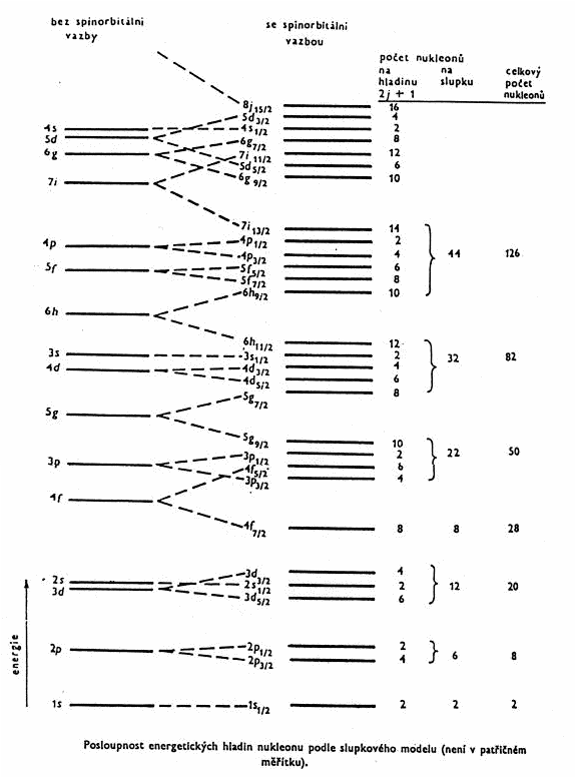
\includegraphics[width=0.6\textwidth]{slupka.png}
	\captionof{figure}{Uspořádání hladin nukleonů v těžkých jádrech popisovaných slupkovým modelem}		
\end{center}

Z něj plynou tyto poznatky: 
\begin{itemize}
	\item Ve srovnání se spektrem energetických hladin atomu vodíku, vzdálenosti mezi hladinami se podstatně nezmenšují s rostoucí energií. To je důsledkem toho, že potenciál prudce klesá se vzdáleností a že se při tom zvyšuje střední vzdálenost nukleonu od centra. Energetické hladiny pro vyšší $l$ leží obecně výše než hladiny pro nižší $l$, což je pochopitelné, neboť člen s orbitálním momentem hybnosti obsažený v SAXON-WOODsově formuli je kladný a nepřevládá nad ním na větších vzdálenostech od centra záporný Coulombický potenciál, který působí na elektrony v atomu.
	
	\item Díky vazbě $\vec{s} \vec{l}$ se hladiny se stejným hlavním kvantovým číslem a stejným vedlejším kvantovým číslem štěpí na dvě, přičemž stav s $j = l - \dfrac{1}{2}$ leží výše než stav s $j = l + \dfrac{1}{2}$. Protože velikost tohoto rozštěpení závisí na $l$, rozštěpení pod vlivem vazby $\vec{s} \vec{l}$ je zvláště patrné u vyšších orbitálních momentů hybnosti.
\end{itemize}	

Slupkový model není vhodný jen k určování energetických hladin, ale dá se využít i ke kvantitativnímu nebo alespoň ke kvalitativnímu určování spinu a magnetických momentů jader (o tom se lze snadno přesvědčit , vyjdeme-li z prostého modelu pracujícího s potenciálem harmonického oscilátoru u lehkých jader).
	

\section{Zobecněný model jádra}

Elementární modely, jimiž jsme se zabývali výše, jsou sice užitečné, neboť podávají fyzikálně podloženou představu o stavbě jádra a umožňují kvantitativně nebo alespoň kvalitativně určit některé jeho vlastnosti. K některým přesnějším studiím však nejsou dost dobré, např. k tomu, aby se určil systém excitovaných hladin nebo chování jádra v jaderných reakcích. 

Jen v některých případech lze nalezené jednonukleonové funkce ve slupkovém modelu jádra použít jako východiska k přesnějšímu teoretickému popisu jádra. Proto bylo vytvořeno více modelů, které jsou vhodnější ke kvantitativnímu vystižení skutečnosti a které poskytují lepší možnosti předpovědět některé vlastnosti jádra nebo průběh jaderných reakcí apod.

Z relativně široké třídy těchto modelů zastávají nejdůležitější místo tzv. zobecněný model, který je určen k popisu a vkladu vlastností daného jádra a optický model, který je užitečný při popisu jaderných reakcí.

Na rozdíl od jednočásticových modelů se v ZOBECNĚNÉM MODELU nepotlačuje zcela přímá interakce mezi nukleony, ale bere se v úvahu.  Přímá interakce mezi nukleony je zodpovědná za to, že se jádro chová také jako celek a jako kolektiv odpovídá na vnější zásah. Projevy jádra jako stmeleného systému vystoupily při štěpení jader, u gigantické rezonance a v široké aplikaci BW formule, vycházející z kapkového modelu jádra. Objeví se ale i jinde.

proto se v zobecněném modelu rozděluje jádro na dva podsystémy. Všechny nukleony ve vnitřních slupkách, které dohromady vytvářejí sudo-sudé jádro, jsou kolektivním podsystémem a zbývající vnější nukleony tvoří podsystém podobný tomu, který známe ze slupkového modelu. Kolektivní podsystém lze pokládat v duchu kapkového modelu za kapku nestlačitelné avšak kvantové kapaliny, která je schopna kvantových oscilací různého typu. V poli tohoto podsystému se potom pohybují v nejjednodušším případě jeden nebo dva nukleony tak, jakoby byly nezávislé.

Energetické spektrum tohoto jádra je v základním stavu v zásadě totožné se spektrem nevzbuzeného jednočásticového modelu. Spektrum vzbuzených stavů se však od spektra jednočásticového modelu liší. Kolektivní podsystém se může excitovat jednak stejně jako jádro u modelu nezávislých částic, jednak jako kapka kvantové kapaliny. Vnější nukleony se excitují stejně jako v modelu nezávislých částic. Energetické spektrum bude nyní bohatší o KOLEKTIVNÍ EXCITACE. Při nich se může měnit také moment hybnosti tohoto podsystému. 

Zobecněný model popisuje dobře spektra, spiny a parity hladin, neboť u jader se skutečně projevují kolektivní excitace. Např. u nuklidu stříbra $^{107}_{47}Ag$ je jeden vnější proton  ve stavu $2p_{1/2}$ a zbytek tvoří sudo-sudý kolektivní podsystém. Jádru v základním stavu přísluší spin a parita $1/2 ^-$. Ve spektru vzbuzeného jádra se jasně projevují kolektivní excitace, které vedou ke stavu se spinem a paritou jádra $3/2 ^-$ a $5/2^-$. 

Dalším prvkem rozšiřujícím možnosti zobecněného modelu je představa, že se dá v souladu s experimentálními daty považovat některý z příslušných kolektivních podsystémů za "jádro", které není sféricky symetrické, ale má jen axiální symetrii. I tyto modely se osvědčují při studiu jader, která jsou axiálně symetrická a nazývají se proto JÁDRY DEFORMOVANÝMI (slupky v takovém jádře jsou napůl obsazené). V tom případě u nich naměříme nenulové el. kvadrupólové momenty.

Základem zobecněného modelu atomového jádra je předpoklad o tom, že jádra vzdálená od magických čísel mají tvar rotačního elipsoidu. Příslušný matematický rozbor vede k závěru, že změna energie takovéhoto jádra může nastat v podstatě trojím způsobem:
\begin{itemize}
	\item změnou stavu některého z vnějších nukleonů (podobně jako u slupkového modelu),
	\item vibrací jádra jako celku $\rightarrow$ $A<150$,
	\item rotací jádra jako celku $\rightarrow$ $A > 150$.
\end{itemize}

U deformovaných jader odpovídají nejnižší vzbuzené energetické hladiny rotačním stavům ($150<A<190$ a $A>220$). Předpokládejme, že jádro má moment setrvačnosti $I$ závislý na excentricitě (tím pádem pro sférická jádra platí $I=0$). Pro sudo-sudá jádra je rotační energie daná vztahem
\begin{equation}
E_{rot} = \dfrac{|\vec{J}|^2}{2I} = \dfrac{\hbar ^2}{2I} (J(J+1)),
\end{equation}
kde $J = 0,2,4,6,...$ je spin jádra, $I$ je moment setrvačnosti. Změřením intervalů mezi energiemi dostaneme moment setrvačnosti $I$. Rotační energie těchto jader jsou rovny
\begin{equation}
E_0 = 0, ~~ E_2 = \dfrac{\hbar ^2}{2I} 6, ~~ E_4 =  \dfrac{\hbar ^2}{2I} 20, ~~ E_6 =  \dfrac{\hbar ^2}{2I}42, ~~ E_8 =  \dfrac{\hbar ^2}{2I} 72, ~~ E_{10} =  \dfrac{\hbar ^2}{2I} 110, ...
\end{equation}
Z teorie tedy dostaneme poměry
\begin{equation}
E_2 : E_4 : E_6: E_8 : E_{10} = 1 :\dfrac{10}{3} : 7:12:\dfrac{55}{3}
\end{equation}
a z experimentu
\begin{equation}
E_2:E_4:E_6:E_8:E_{10} = 1:3,32:6,92:11,7:17,6.
\end{equation}

Pozn.: šišaté jádro nelze otáčet kolem osy rotace.
\begin{itemize}
	\item často používaný nesférický deformovaný potenciál - Nilssonův potenciál
	\item deformovaný potenciál $\rightarrow$ energie jednočásticových hladin závisí na velikosti deformace
	\item interakce mezi kolektivními a jednočásticovými stavy $\rightarrow$směs různých stavů
	\item vzniká složitý systém jednočásticových, vibračních a rotačních stavů (hladin)
\end{itemize}

ZOBECNĚNÝ MODEL DOKÁŽE DOBŘE POPSAT SLOŽITÝ SYSTÉM ENERGETICKÝCH HLADIN V JÁDŘE, CHARAKTERISTIKY STAVŮ, PRAVDĚPODOBNOSTI PŘECHODŮ MEZI NIMI A KVADRUPÓLOVÉ MOMENTY JADER.

\subsection{Optický model}

Tento model popisuje efekty jádra na příchozí částici při jaderných reakcích s pomocí potenciálové jámy, která má schopnost absorpce: díky tomuto potenciálu lze proces popsat řešením Schr$\ddot{o}$dingerovy rovnice pro volné stavy příchozí částice.

Uveďme příklad potenciálu optického modelu pro rozptyl neutronu a protonu na jádře
\begin{equation}
V(r) = V_c (r) - V f_1 (r) - iWf_2(r) + V_{LS} \left( \dfrac{\hbar}{m_{\pi} c} \right) \dfrac{1}{r} \dfrac{d f_{LS}(r)}{dr} \vec{L} \cdotp \vec{S}, 
\end{equation}
kde $V_c$ je Coulombický potenciál pro proton, $V f_1$ je jaderná potenciálová jáma, $i W f_2$ je imaginární potenciál reprezentující absorpci příchozího nukleonu a poslední člen reprezentuje spin-orbitální interakci. $V, W$ a $V_{LS}$ se mění s energií. Faktor $(\hbar /m_{\pi}c)^2$ má rozměr plochy a vyruší tak dva rozměry délky pocházející z následujícího faktoru v daném členu. faktory $f_1, f_2$ a $f_{LS}$ jsou obvykle voleny ve Saxon-Woodsově tvaru.


Další modely jader: 
\begin{itemize}
	\item velmi silný vliv párování, pár nukleonů může být natolik silně vázán, že se na něj můžeme  dívat jako na jednu částici (spiny dvou fermionů se složí $\rightarrow$ boson). Na tom je založen MODEL INTERAGUJÍCÍCH BOSONŮ (IBA).
	\item Silné párování je základem i MODELŮ NEZÁVISLÝCH KVAZIČÁSTIC.
	\item MIKROSKOPICKÉ MODELY vycházející z nukleonového potenciálu a řešící pohybové rovnice $\rightarrow$ problémy s matematickým řešením.
\end{itemize}	
  
\end{document}